\chapter{Site Web}

\section{Objectifs}

Le site web fut principalement un moyen de présenter, de façon graphique, le résultat des différentes partie abordées durant ce projet. Pour la première partie, il consistait à afficher, grâce à l'utilisation des diagrammes, les statistiques de notre étude sur les certificats. La deuxième partie tourne plus autour de l'audit. Nous avons souhaité présenter un résumé de notre rapport d'audit, qui a était livré lors de la deuxième livraison. Enfin, notre site fut aussi une plate-forme pour l'intégration de la troisième partie du projet qui consiste à tester la navigateur client. \\


\section{Statistiques}

Après certaine recherche, nous nous sommes mis d'accord sur l'utilisation de l'application javascript \textit{Highcharts} pour la représentation des différents diagrammes sur le site. L'utilisation reste simple et varier. Il fut possible de l'utiliser de 3 façon différentes : 
\begin{itemize}
\item \textbf{Statique} : données sont récupérées directement depuis un tableau HTML;
\item \textbf{Dynamique} : données sont récupérer depuis la base de données;
\item \textbf{AJAX} : données sont récupérer par des appels AJAX\\
\end{itemize}

Chaque diagrammes possèdent une fonctionnalité \textit{tooltip} qui offre plus d'information sur les données représenter. Il est actionné lors du passage de la souris sur une part du cadre du diagramme circulaire (voir figure \ref{taille_clefs})

\subsection{Statistiques Générales}

Nous avons souhaité faire une comparaison entre les deux scans réaliser durant le développement de la première partie du projet. De ce fait, nous présentons sur un même diagramme la proportion des certificats récupérer et les certificats qui y sont vulnérables pour le premier et deuxième scan. On y affiche également un tableau contenant, en chiffres, les valeurs du diagramme ainsi que le pourcentage des certificats vulnérables par rapport au certificats récupérés.

\begin{figure}[H]
\begin{center}
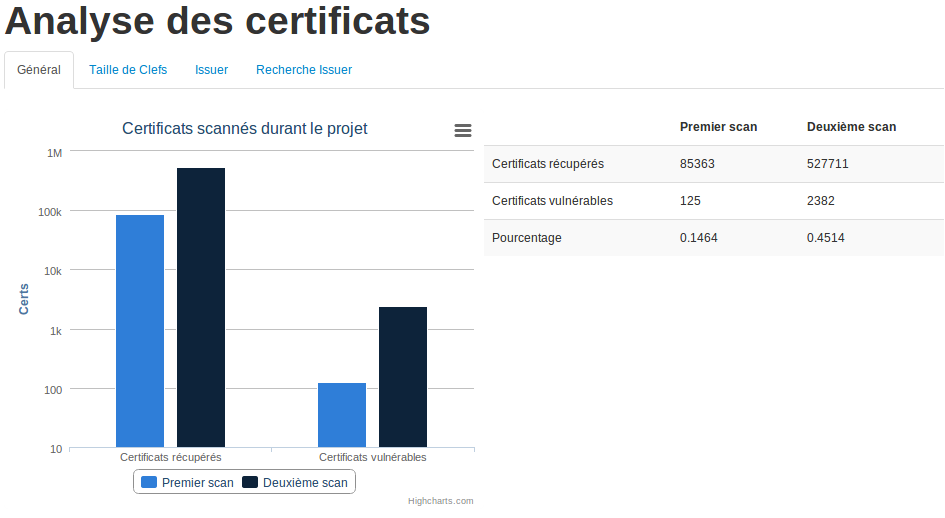
\includegraphics[scale=0.5]{images/site_web_stats_gen.png}
\end{center}
\caption{Site Web - Statistique Général}
\label{stats_general}
\end{figure}

\subsection{Taille des clefs}

On représente ici, avec un diagramme circulaire, les tailles des clefs des certificats récupérés. De tout les certificats se trouvant sur notre base de données, on identifie ceux possédant une taille de clef commençant de 512o à 16384o.

\begin{figure}[H]
\begin{center}
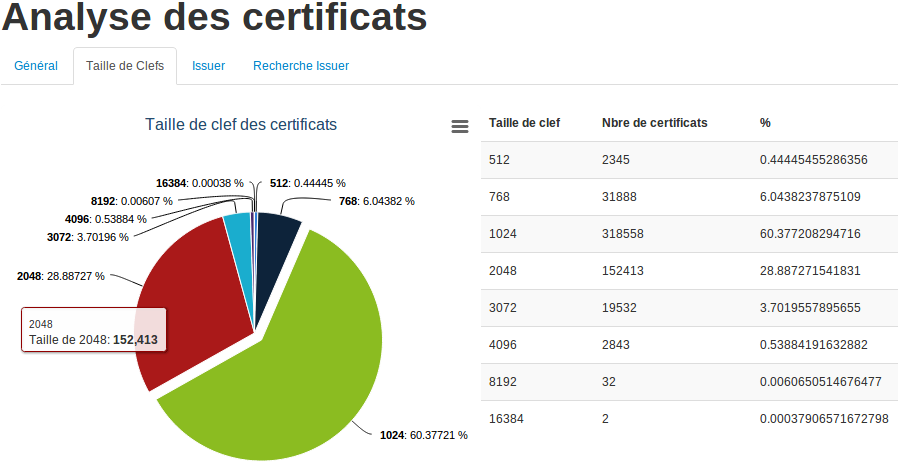
\includegraphics[scale=0.5]{images/site_web_stats_clefs.png}
\end{center}
\caption{Site Web - Taille de clef}
\label{taille_clefs}
\end{figure}

\subsection{Les émetteurs}

Cette partie concerne plutôt un tableau représentatif de tout les émetteurs se trouvant sur notre base de données. On y récupère aussi, par deux requêtes SQL le nombre total de certificats qui possèdent chaque émetteur ainsi que le nombre de certificats qui y sont vulnérables.

\begin{figure}[H]
\begin{center}
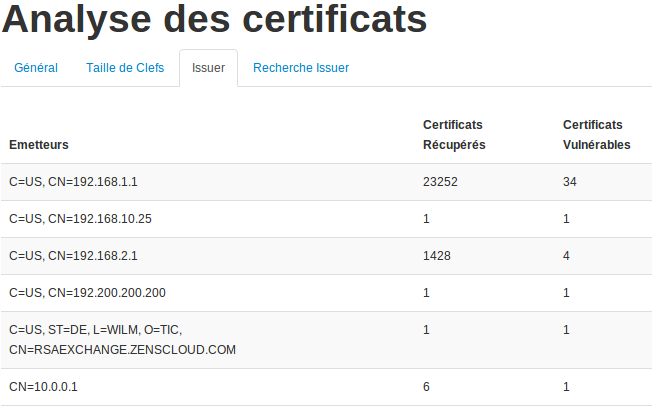
\includegraphics[scale=0.5]{images/site_web_issuer.png}
\end{center}
\caption{Site Web - Emetteurs}
\label{issuer}
\end{figure}

\subsection{Onglet de recherche}

Nous avons également intégré un outil de recherche de certificats. L'utilisateur peut faire des recherches en se basant sur les trois critères suivantes :
\begin{itemize}
\item Le sujet (\textit{subject}) se trouvant sur le certificat,
\item L'émetteur (\textit{issuer}),
\item et la taille de la clef\\
\end{itemize}

\begin{figure}[H]
\begin{center}
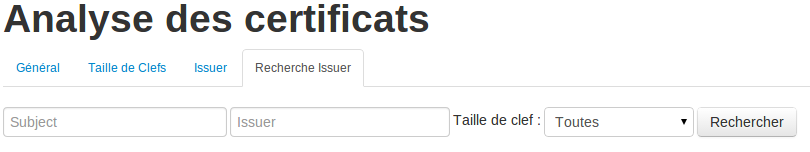
\includegraphics[scale=0.5]{images/site_web_search_bar.png}
\end{center}
\caption{Site Web - Bar de recherche}
\label{search_bar}
\end{figure}

La requête est envoyé sur le serveur par un appel en AJAX et le résultat est affiché avec un diagramme circulaire en représentant le nombre total de certificats retrouvés en base et le nombre de certificats vulnérables.

\begin{figure}[H]
\begin{center}
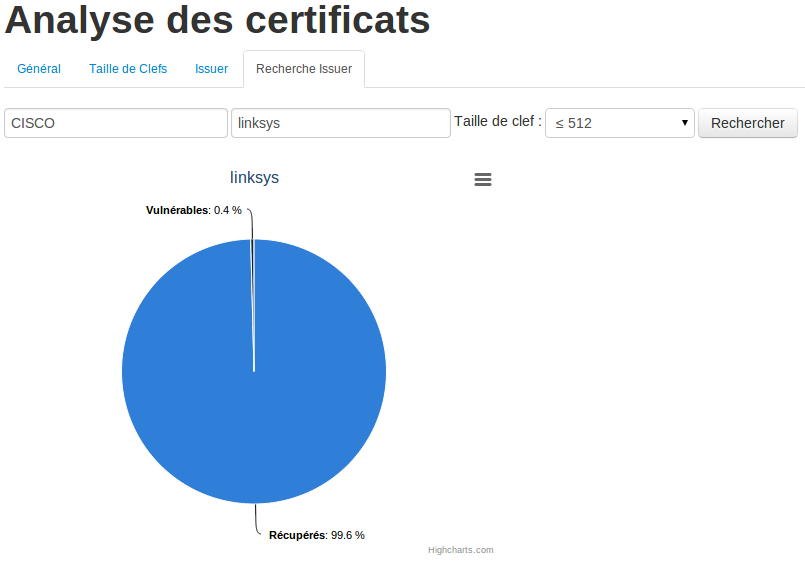
\includegraphics[scale=0.5]{images/site_web_search_result.png}
\end{center}
\caption{Site Web - Résultat d'une recherche}
\label{search_result}
\end{figure}

 
\section{Résumé d'audit}

Nous représentons dans cette partie, une résumé des sections abordées dans le rapport d'audit. Le but étant de garder une structure d'audit dans le groupe.


\section{Test Navigateur Client}

Cette partie intègre l'outil permettant d'analyser les différentes \textit{ciphersuite} utilisées à l'établissement de connexion d'un client à un serveur, comme expliqué au chapitre \ref{analyseDynamique}. La page est divisé en 4 tableaux :
\begin{itemize}
\item Version et Algorithmes de chiffrement supportées
\item Algorithmes de signatures,
\item Courbes elliptiques
\item Légende\\
\end{itemize}

\begin{figure}[H]
\begin{center}
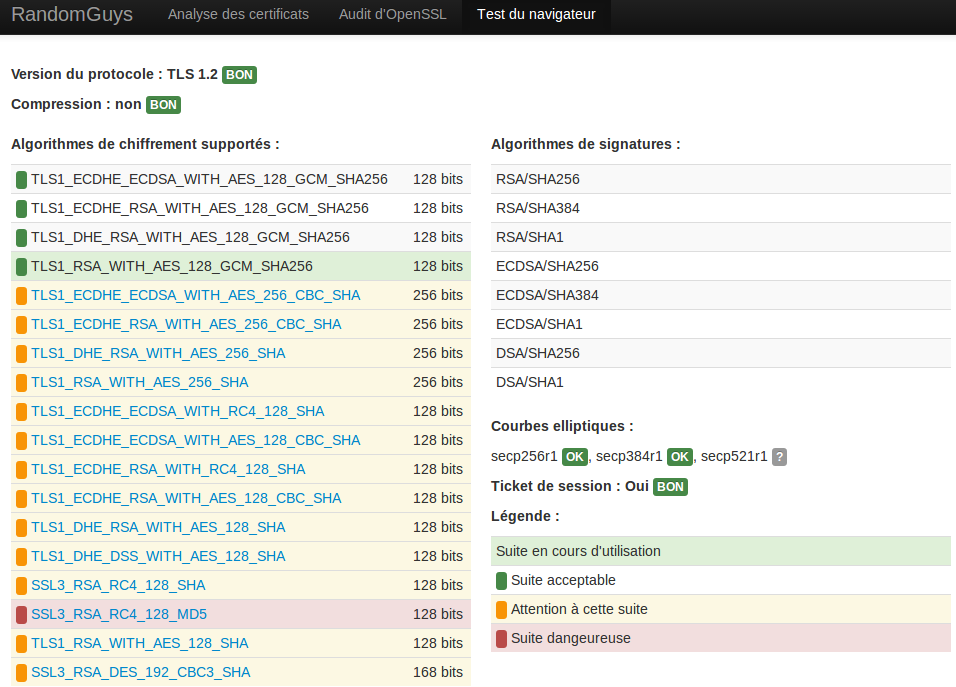
\includegraphics[scale=0.5]{images/site_web_test_client.png}
\end{center}
\caption{Site Web - Test du Navigateur}
\label{test_client}
\end{figure}

